%-----------------------------------------------------------------------------------------------------------------------------------------------%
%	The MIT License (MIT)
%
%	Copyright (c) 2019 Jan Küster
%
%	Permission is hereby granted, free of charge, to any person obtaining a copy
%	of this software and associated documentation files (the "Software"), to deal
%	in the Software without restriction, including without limitation the rights
%	to use, copy, modify, merge, publish, distribute, sublicense, and/or sell
%	copies of the Software, and to permit persons to whom the Software is
%	furnished to do so, subject to the following conditions:
%	
%	THE SOFTWARE IS PROVIDED "AS IS", WITHOUT WARRANTY OF ANY KIND, EXPRESS OR
%	IMPLIED, INCLUDING BUT NOT LIMITED TO THE WARRANTIES OF MERCHANTABILITY,
%	FITNESS FOR A PARTICULAR PURPOSE AND NONINFRINGEMENT. IN NO EVENT SHALL THE
%	AUTHORS OR COPYRIGHT HOLDERS BE LIABLE FOR ANY CLAIM, DAMAGES OR OTHER
%	LIABILITY, WHETHER IN AN ACTION OF CONTRACT, TORT OR OTHERWISE, ARISING FROM,
%	OUT OF OR IN CONNECTION WITH THE SOFTWARE OR THE USE OR OTHER DEALINGS IN
%	THE SOFTWARE.
%	
%
%-----------------------------------------------------------------------------------------------------------------------------------------------%


%============================================================================%
%
%	DOCUMENT DEFINITION
%
%============================================================================%

%we use article class because we want to fully customize the page and don't use a cv template
\documentclass[10pt,A4]{article}	


%----------------------------------------------------------------------------------------
%	ENCODING
%----------------------------------------------------------------------------------------

% we use utf8 since we want to build from any machine
\usepackage[utf8]{inputenc}		

%----------------------------------------------------------------------------------------
%	LOGIC
%----------------------------------------------------------------------------------------

% provides \isempty test
\usepackage{xstring, xifthen}

%----------------------------------------------------------------------------------------
%	FONT BASICS
%----------------------------------------------------------------------------------------

% some tex-live fonts - choose your own

%\usepackage[defaultsans]{droidsans}
%\usepackage[default]{comfortaa}
%\usepackage{cmbright}
\usepackage[default]{raleway}
%\usepackage{fetamont}
%\usepackage[default]{gillius}
%\usepackage[light,math]{iwona}
%\usepackage[thin]{roboto} 

% set font default
\renewcommand*\familydefault{\sfdefault} 	
\usepackage[T1]{fontenc}

% more font size definitions
\usepackage{moresize}

%----------------------------------------------------------------------------------------
%	FONT AWESOME ICONS
%---------------------------------------------------------------------------------------- 

% include the fontawesome icon set
\usepackage{fontawesome}

% use to vertically center content
% credits to: http://tex.stackexchange.com/questions/7219/how-to-vertically-center-two-images-next-to-each-other
\newcommand{\vcenteredinclude}[1]{\begingroup
\setbox0=\hbox{\includegraphics{#1}}%
\parbox{\wd0}{\box0}\endgroup}

% use to vertically center content
% credits to: http://tex.stackexchange.com/questions/7219/how-to-vertically-center-two-images-next-to-each-other
\newcommand*{\vcenteredhbox}[1]{\begingroup
\setbox0=\hbox{#1}\parbox{\wd0}{\box0}\endgroup}

% icon shortcut
\newcommand{\icon}[3] { 							
	\makebox(#2, #2){\textcolor{maincol}{\csname fa#1\endcsname}}
}	

% icon with text shortcut
\newcommand{\icontext}[4]{ 						
	\vcenteredhbox{\icon{#1}{#2}{#3}}  \hspace{2pt}  \parbox{0.9\mpwidth}{\textcolor{#4}{#3}}
}

% icon with website url
\newcommand{\iconhref}[5]{ 						
    \vcenteredhbox{\icon{#1}{#2}{#5}}  \hspace{2pt} \href{#4}{\textcolor{#5}{#3}}
}

% icon with email link
\newcommand{\iconemail}[5]{ 						
    \vcenteredhbox{\icon{#1}{#2}{#5}}  \hspace{2pt} \href{mailto:#4}{\textcolor{#5}{#3}}
}

%----------------------------------------------------------------------------------------
%	PAGE LAYOUT  DEFINITIONS
%----------------------------------------------------------------------------------------

% page outer frames (debug-only)
% \usepackage{showframe}

% we use paracol to display breakable two columns
\usepackage{paracol}

% define page styles using geometry
\usepackage[a4paper]{geometry}

% remove all possible margins
\geometry{top=1cm, bottom=1cm, left=1cm, right=1cm}

\usepackage{fancyhdr}
\pagestyle{empty}

% space between header and content
% \setlength{\headheight}{0pt}

% indentation is zero
\setlength{\parindent}{0mm}

%----------------------------------------------------------------------------------------
%	TABLE /ARRAY DEFINITIONS
%---------------------------------------------------------------------------------------- 

% extended aligning of tabular cells
\usepackage{array}

% custom column right-align with fixed width
% use like p{size} but via x{size}
\newcolumntype{x}[1]{%
>{\raggedleft\hspace{0pt}}p{#1}}%


%----------------------------------------------------------------------------------------
%	GRAPHICS DEFINITIONS
%---------------------------------------------------------------------------------------- 

%for header image
\usepackage{graphicx}

% use this for floating figures
% \usepackage{wrapfig}
% \usepackage{float}
% \floatstyle{boxed} 
% \restylefloat{figure}

%for drawing graphics		
\usepackage{tikz}				
\usetikzlibrary{shapes, backgrounds,mindmap, trees}

%----------------------------------------------------------------------------------------
%	Color DEFINITIONS
%---------------------------------------------------------------------------------------- 
\usepackage{transparent}
\usepackage{color}

% primary color
\definecolor{maincol}{RGB}{ 150, 150, 255 }

% accent color, secondary
\definecolor{accentcol}{RGB}{ 50, 50, 100 }


% dark color
\definecolor{darkcol}{RGB}{ 70, 70, 70 }

% light color
\definecolor{lightcol}{RGB}{245,245,245}


% Package for links, must be the last package used
\usepackage[hidelinks]{hyperref}

% returns minipage width minus two times \fboxsep
% to keep padding included in width calculations
% can also be used for other boxes / environments
\newcommand{\mpwidth}{\linewidth-\fboxsep-\fboxsep}
	


%============================================================================%
%
%	CV COMMANDS
%
%============================================================================%

%----------------------------------------------------------------------------------------
%	 CV LIST
%----------------------------------------------------------------------------------------

% renders a standard latex list but abstracts away the environment definition (begin/end)
\newcommand{\cvlist}[1] {
	\begin{itemize}{#1}\end{itemize}
}

%----------------------------------------------------------------------------------------
%	 CV TEXT
%----------------------------------------------------------------------------------------

% base class to wrap any text based stuff here. Renders like a paragraph.
% Allows complex commands to be passed, too.
% param 1: *any
\newcommand{\cvtext}[1] {
	\begin{tabular*}{1\mpwidth}{p{0.98\mpwidth}}
		\parbox{1\mpwidth}{#1}
	\end{tabular*}
}

%----------------------------------------------------------------------------------------
%	CV SECTION
%----------------------------------------------------------------------------------------

% Renders a a CV section headline with a nice underline in main color.
% param 1: section title
\newcommand{\cvsection}[1] {
	%\vspace{14pt}
	\cvtext{
		\textbf{\LARGE{\textcolor{darkcol}{\uppercase{#1}}}}\\[-4pt]
		\textcolor{maincol}{ \rule{0.1\textwidth}{2pt} } \\
	}
}

%----------------------------------------------------------------------------------------
%	META SKILL
%----------------------------------------------------------------------------------------

% Renders a progress-bar to indicate a certain skill in percent.
% param 1: name of the skill / tech / etc.
% param 2: level (for example in years)
% param 3: percent, values range from 0 to 1
% \newcommand{\cvskill}[3] {
% 	\begin{tabular*}{1\mpwidth}{p{0.72\mpwidth}  r}
%  		\textcolor{black}{\textbf{#1}} & \textcolor{maincol}{#2}\\
% 	\end{tabular*}%
	
% 	\hspace{4pt}
% 	\begin{tikzpicture}[scale=1,rounded corners=2pt,very thin]
% 		\fill [lightcol] (0,0) rectangle (1\mpwidth, 0.15);
% 		\fill [maincol] (0,0) rectangle (#3\mpwidth, 0.15);
%   	\end{tikzpicture}%
% }
\newcommand{\cvskill}[3] {
	\begin{tabular*}{1\mpwidth}{p{0.99\mpwidth}  r}
 		\textcolor{black}{\textbf{#1}} & \textcolor{maincol}{#2}\\[-10pt]
	\end{tabular*}%
    
	\hspace{4pt}
	\begin{tikzpicture}[scale=1,rounded corners=2pt,very thin]
		\fill [lightcol] (0,0) rectangle (1\mpwidth, 0.15);
		\fill [maincol] (0,0) rectangle (#3\mpwidth, 0.15);
  	\end{tikzpicture}%
}


%----------------------------------------------------------------------------------------
%	 CV EVENT
%----------------------------------------------------------------------------------------

% Renders a table and a paragraph (cvtext) wrapped in a parbox (to ensure minimum content
% is glued together when a pagebreak appears).
% Additional Information can be passed in text or list form (or other environments).
% the work you did
% param 1: time-frame i.e. Sep 14 - Jan 15 etc.
% param 2:	 event name (job position etc.)
% param 3: Customer, Employer, Industry
% param 4: Short description
% param 5: work done (optional)
% param 6: technologies include (optional)
% param 7: achievements (optional)
\newcommand{\cvevent}[7] {
	
	% we wrap this part in a parbox, so title and description are not separated on a pagebreak
	% if you need more control on page breaks, remove the parbox
	\parbox{\mpwidth}{
		\begin{tabular*}{1\mpwidth}{p{0.72\mpwidth}  r}
	 		\textcolor{black}{\textbf{#2}} & \colorbox{maincol}{\makebox[0.25\mpwidth]{\textcolor{white}{#1}}} \\
			\textcolor{maincol}{\textbf{#3}} & \\
		\end{tabular*}\\[8pt]
	
		\ifthenelse{\isempty{#4}}{}{
			\cvtext{#4}\\
		}
	}

	\ifthenelse{\isempty{#5}}{}{
		\vspace{9pt}
		{#5}
	}

	\ifthenelse{\isempty{#6}}{}{
		\vspace{9pt}
		\cvtext{\textbf{Technologies include:}}\\
		{#6}
	}

	\ifthenelse{\isempty{#7}}{}{
		\vspace{9pt}
		\cvtext{\textbf{Achievements include:}}\\
		{#7}
	}
	\vspace{14pt}
}

%----------------------------------------------------------------------------------------
%	 CV META EVENT
%----------------------------------------------------------------------------------------

% Renders a CV event on the sidebar
% param 1: title
% param 2: subtitle (optional)
% param 3: customer, employer, etc,. (optional)
% param 4: info text (optional)
\newcommand{\cvmetaevent}[4] {
	\textcolor{maincol} {\cvtext{\textbf{\begin{flushleft}#1\end{flushleft}}}}

	\ifthenelse{\isempty{#2}}{}{
	\textcolor{darkcol} {\cvtext{\textbf{#2}} }
	}

	\ifthenelse{\isempty{#3}}{}{
		\cvtext{{ \textcolor{darkcol} {#3} }}\\
	}

	\cvtext{#4}\\[14pt]
}

%---------------------------------------------------------------------------------------
%	QR CODE
%----------------------------------------------------------------------------------------

% Renders a qrcode image (centered, relative to the parentwidth)
% param 1: percent width, from 0 to 1
\newcommand{\cvqrcode}[1] {
	\begin{center}
		
\includegraphics[width={#1}\mpwidth]{qrcode}
	\end{center}
}

\begin{document}

%============================================================================%
%
%
%
%	DOCUMENT CONTENT
%
%
%
%============================================================================%
\columnratio{0.31}
\setlength{\columnsep}{2.2em}
\setlength{\columnseprule}{4pt}
\colseprulecolor{lightcol}
\begin{paracol}{2}
    \begin{leftcolumn}
    %---------------------------------------------------------------------------------------
    %	META IMAGE
    %----------------------------------------------------------------------------------------
    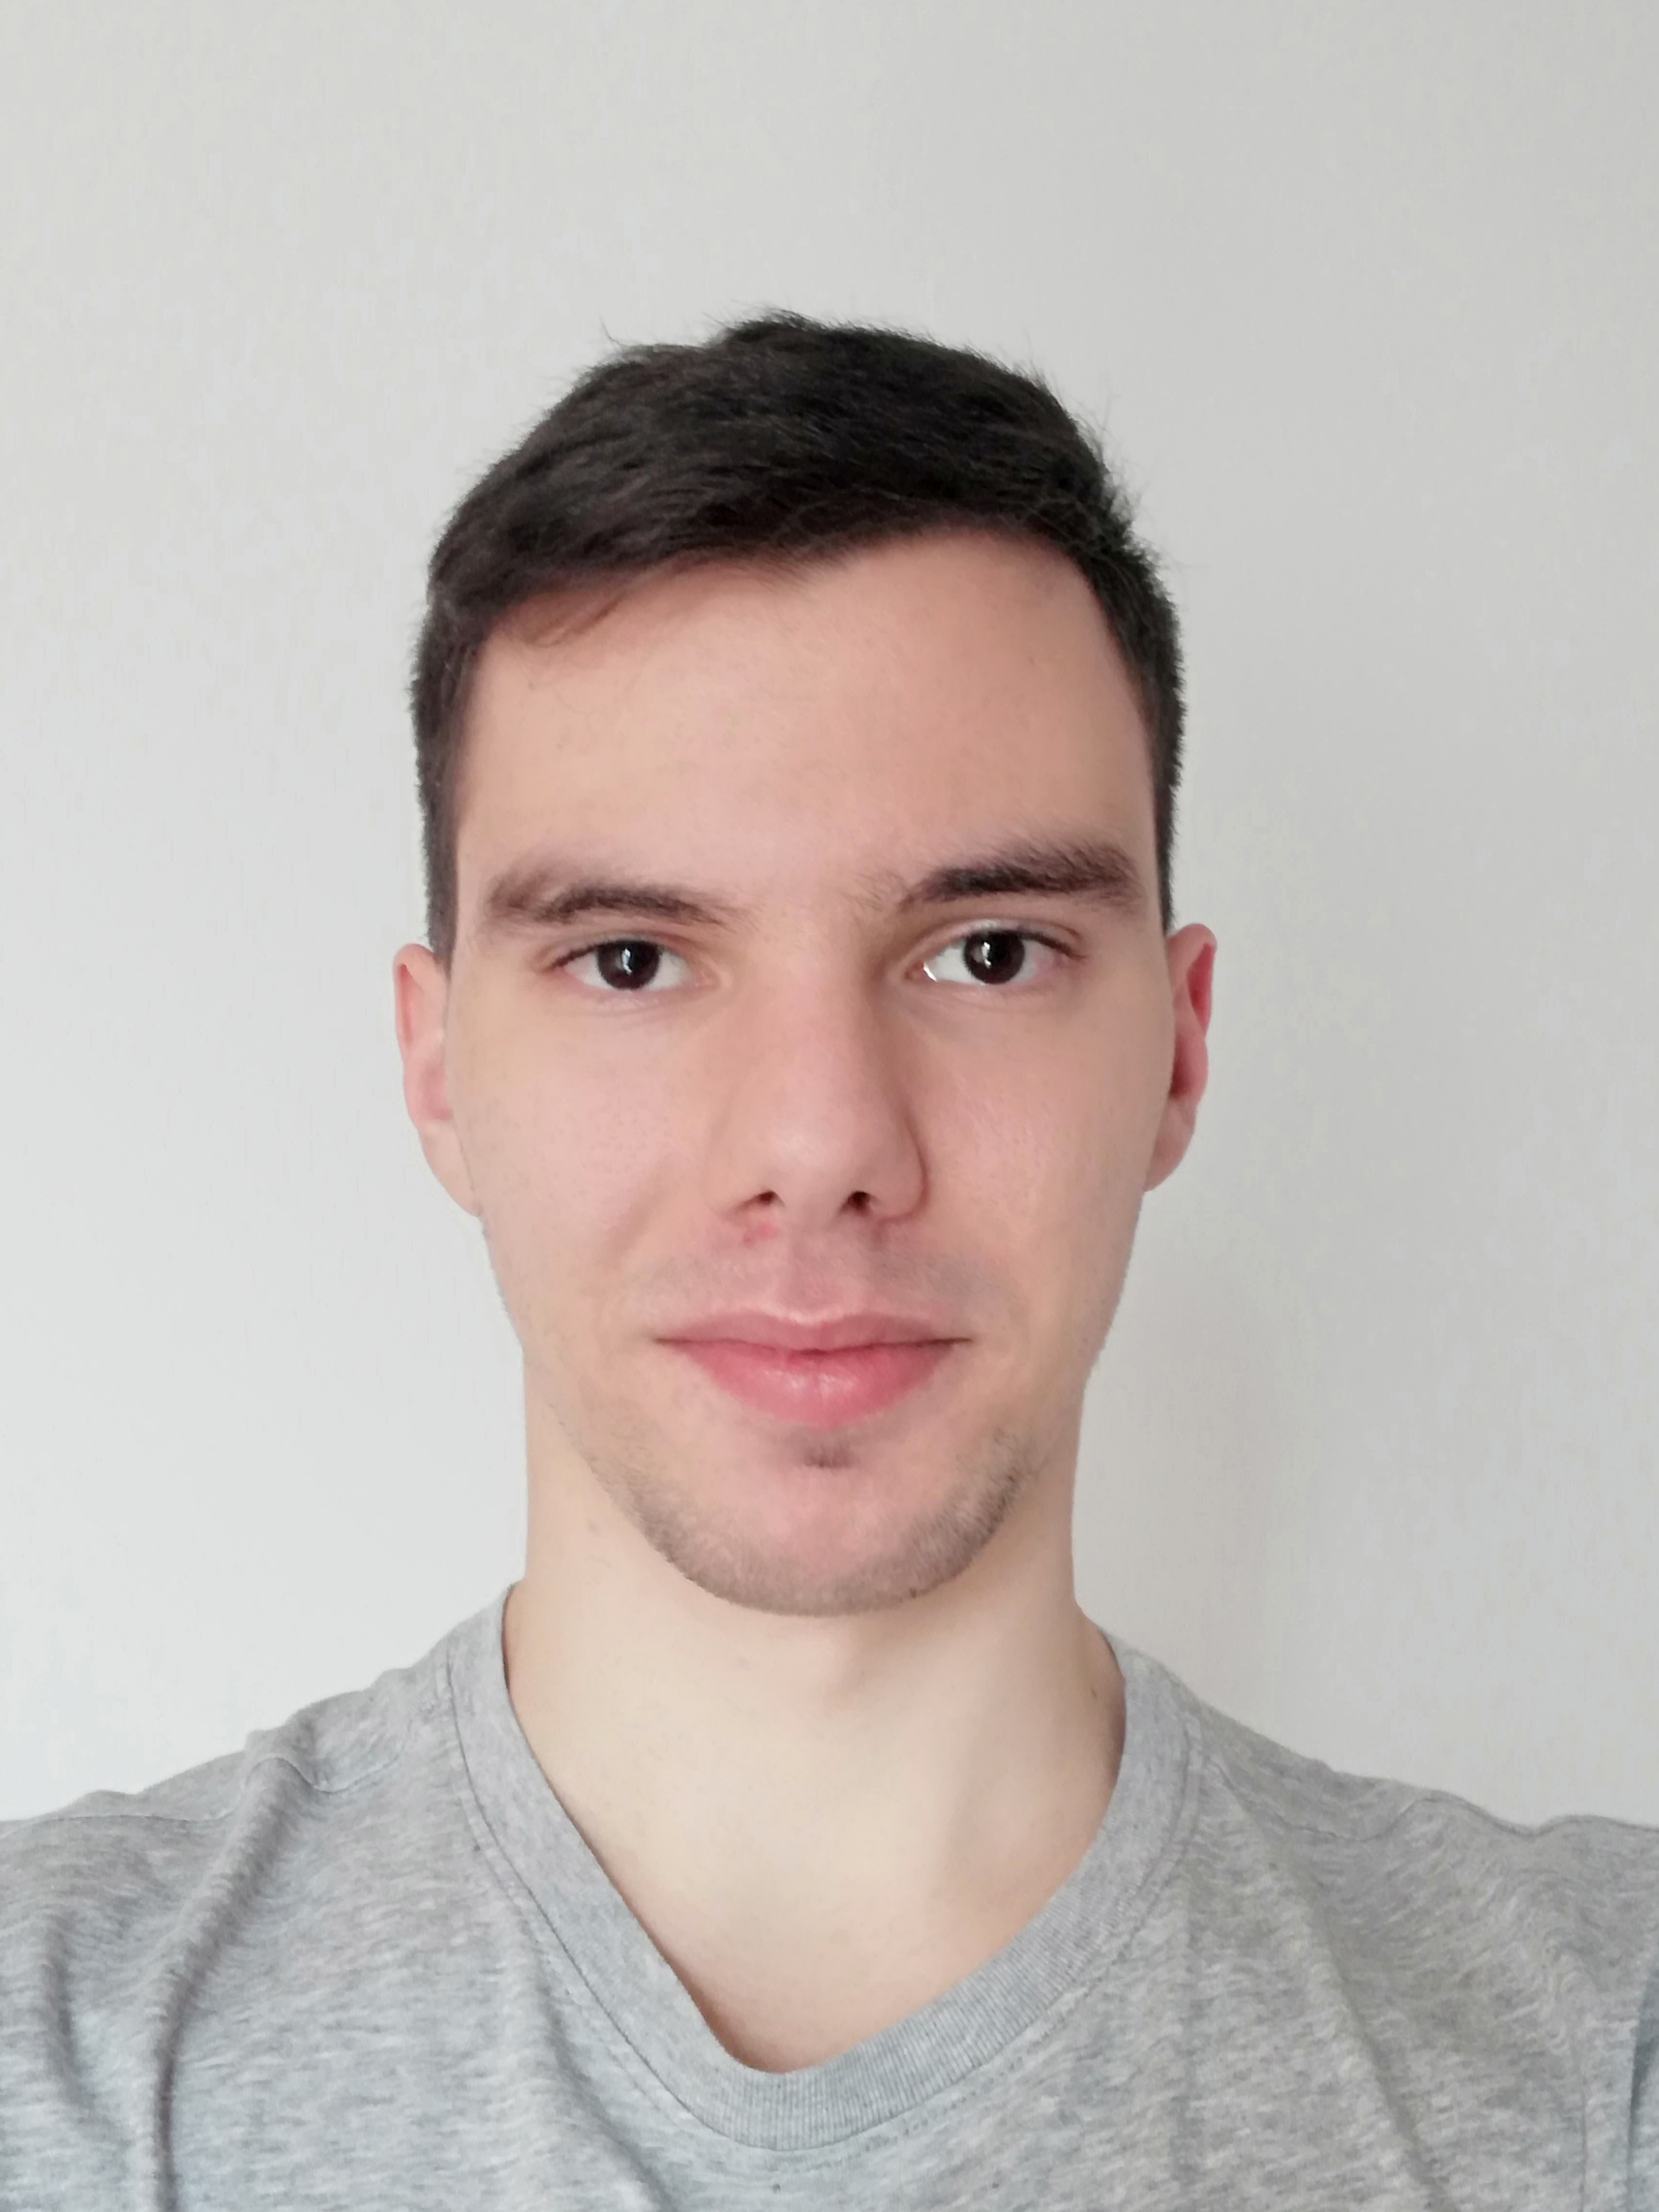
\includegraphics[width=\linewidth]{IMG_20220519_174910.jpg}	%trimming relative to image size
    
    %---------------------------------------------------------------------------------------
    %	META SKILLS
    %----------------------------------------------------------------------------------------

    \vfill\null
    \cvsection{SKILLS}

    \cvskill{Python}{}{1} \\
    \cvskill{SQL}{}{0.9} \\
    \cvskill{C}{}{0.8} \\
    \cvskill{Java}{}{0.8} \\
    \cvskill{C++}{}{0.75} \\
    \cvskill{R}{}{0.65} \\
    \cvskill{JavaScript}{}{0.5} \\
    
    \cvskill{SQL Server Management Studio}{}{0.86} \\
    \cvskill{AWS}{}{0.7} \\
    \cvskill{Pentaho}{}{0.5} \\
    \cvskill{ArchiMate}{}{0.45} \\
    \cvskill{Camunda Modeler}{}{0.4} \\
    \cvskill{Enterprise Architect}{}{0.4} \\

    \vfill\null
    \cvsection{CONTACTS}
    
    \cvtext{
    \begin{tabular}{ m{0.01cm} l }
    \faPhone & +351 935 570 378 \\ 
    \href{mailto:pro.joaoarcosta@gmail.pt}{\faEnvelope} &
    \href{mailto:pro.joaoarcosta@gmail.pt}{pro.joaoarcosta@gmail.pt} \\  
    \href{https://linkedin.com/in/jarcosta/}{\faLinkedin} &
    \href{https://linkedin.com/in/jarcosta/}{www.linkedin.com/in/jarcosta} \\
    \href{https://github.com/jarcosta}{\faGithub} &
    \href{https://github.com/jarcosta}{www.github.com/jarcosta}
    \end{tabular}
    }
    
    \newpage
    \cvsection{HOBBIES}
    
    \cvmetaevent
    {Projects and Practical Experience}
    {}
    {}
    {In my free time, I have developed various personal projects, showcased on my \textbf{GitHub}, that involve \textbf{API} integrations, \textbf{data handling}, and \textbf{decision-making algorithms}.
    
    Additionally, I am self-taught in \textbf{Excel}, which I regularly use to streamline and automate tasks.
    }
    
    \cvmetaevent
    {Sports}
    {}
    {}
    {Swimming, Cycling, \\Snowboarding, Basketball}
    
    %---------------------------------------------------------------------------------------
    %	CERTIFICATION
    %----------------------------------------------------------------------------------------
    %\newpage
    \vfill\null
    \cvsection{CERTIFICATIONS}
    
    \cvmetaevent
    {Cambridge English}
    {C1 Advanced Exam}
    {}
    {Score: 171}
    
    \cvmetaevent
    {ABC bootcamps}
    {English summer course}
    {Edinburgh}
    {A two-week intensive English course in Edinburgh, where I developed my independence, communication and cooperation skills.}
    
    \cvmetaevent
    {Udemy}
    {2D Game online course development}
    {}
    {\textcolor{maincol}{\href{https://udemy-certificate.s3.amazonaws.com/pdf/UC-d7553e16-cd48-4367-a447-73e2f10a2d3a.pdf}{(certificate)}}}
    
    %\newpage
    %\mbox{} % hotfix to place qrcode on the bottom when there are not other elements
    %\vfill
    %\cvqrcode{0.7}
    
    \end{leftcolumn}
\begin{rightcolumn}
    %---------------------------------------------------------------------------------------
    %	TITLE  HEADER
    %----------------------------------------------------------------------------------------
    \fcolorbox{white}{accentcol}{\begin{minipage}[c][3.5cm][c]{1\mpwidth}
        \begin {center}
            \HUGE{ \textbf{ \textcolor{white}{ \uppercase{ João Roque Costa } } } } \\[-24pt]
            \textcolor{white}{ \rule{0.1\textwidth}{1.25pt} } \\[4pt]
            \large{ \textcolor{white} {Coimbra, Portugal} }
        \end {center}
    \end{minipage}} \\[14pt]
    \vspace{-12pt}
    
    %---------------------------------------------------------------------------------------
    %	PROFILE
    %----------------------------------------------------------------------------------------
    \vfill\null
    
%    \cvtext{
%    A Master's student in Computer Science at IST with a strong interest in \textbf{problem-solving}, \textbf{financial markets}, \textbf{artificial intelligence}, and \textbf{data science}.\\ \\
%    Eager to join a dynamic team, enhance my skills, and tackle new challenges in the IT industry. \\ \\
%    }

    %---------------------------------------------------------------------------------------
    %	WORK EXPERIENCE
    %----------------------------------------------------------------------------------------
    \vfill\null
    \cvsection{WORK EXPERIENCE}

    \cvevent
        {Oct 24 - Jan 25}
        {Teaching Assistant – Data Science}
        {Instituto Superior Técnico}
        {Invited to work as a Teaching Assistant for the \textbf{Data Science} course, where I was responsible for guiding students through practical lab sessions.}
        {}
        {}
        {}
    
    \vfill\null
    \cvevent
        {July 2018}
        {Software Development Intern}
        {\href{https://mariaadelaide.com/}{Maria Adelaide} and \href{http://playsketch.net}{Playsketch}}
        {Key contributions:{\cvlist{
            \item Developed and optimized the \textbf{email automation system}, improving workflow efficiency.
            \item After completing my work on the email automation system, I was awarded a \textbf{game development course}, where I built a \textbf{Space Invaders} clone and a \textbf{Number Wizard} game for mobile devices.
        }}}
        {}
        {}
        {}

   %---------------------------------------------------------------------------------------
   %	EDUCATION
   %----------------------------------------------------------------------------------------
   \vfill\null
   \cvsection{EDUCATION}


    \cvevent
        {Sep 23 - NOW}
        {M. Sc. Computer Science and Engineering}
        {Instituto Superior Técnico}
        {
        A two-year program where I chose to focus in:
        {\cvlist{
            \item \textbf{Machine Learning}: Deep Learning, Agent Learning, Multi-Agent Systems, Intelligent Decision Making
            \item \textbf{Data Science}: Data Visualization, Data Analysis, Data Integration
            \item \textbf{Cloud Computing}
            \item \textbf{Information Systems}
        }}
        I am currently writing my thesis on \textbf{Dimensionality Reduction on Disjoint Manifolds}. To complement my research, I enrolled in the \textbf{Optimization and Algorithms} course as an elective within my curriculum. Additionally, I plan to apply for publication with the \textbf{Association for the Advancement of Artificial Intelligence (AAAI)}.
        }
        {}
        {\cvlist{
            \item \textbf{Machine Learning and Data Science}: Sklearn, pandas, numpy;
            \item \textbf{Cloud Computing}: AWS;
            \item \textbf{Information Systems}: CmapTools, SQL Server Management Studio, \\Pentaho.
        }}
        {}

    \vfill\null
    \cvevent
        {Sep 20 – Jul 23}
        {B. Sc. in Computer Science and Engineering}
        {Instituto Superior Técnico}
        {Throughout my bachelor's degree, I worked on various projects that strengthened both my technical expertise and teamwork skills. Key areas of study and practical experience include:}
        {\cvlist{
            \item \textbf{Mathematics and Foundations}: \textbf{Differential and Integral Calculus}, \textbf{Physics}, \textbf{Linear Algebra}, \textbf{Discrete Mathematics}, \textbf{Probability and Statistics}, which later proved useful in my thesis research.
            \item \textbf{Low-Level Computing}: \textbf{Compilers}, \textbf{Operating Systems}, \textbf{Distributed Systems}, \textbf{Computer Architecture}, and \textbf{Computer Networks}, providing a solid understanding of system architecture and performance.
            \item \textbf{Data Science and Artificial Intelligence}: \textbf{Artificial Intelligence}, \textbf{Databases}, and \textbf{Machine Learning}, which sparked my interest and led me to further specialize in this area during my master's degree.
            \item \textbf{Management}: Developed foundational knowledge of company economics through the \textbf{Management} course.
        }}
        {\cvlist{
            \item \textbf{Database Management}: SQL for data storage and querying.
            \item \textbf{Systems Modeling}: \textbf{ArchiMate}, \textbf{Camunda Modeler}, and \textbf{Enterprise Architect (Sparx)}.
            \item \textbf{Programming}: \textbf{JavaScript} for human-computer interaction and computer graphics, \textbf{Python} (\textbf{NumPy, Pandas}) for machine learning, and \textbf{Java} for software development.
        }}
        {\cvlist{
            \item \textbf{Project Management and Teamwork}: Learned to effectively distribute tasks, collaborate on complex projects, and develop persistence in problem-solving.
        }}

    % hotfixes to create fake-space to ensure the whole height is used
    \mbox{}
    \vfill
    \mbox{}
    \vfill
    \mbox{}
    \vfill
    \mbox{}
    \end{rightcolumn}
    
\end{paracol}

\end{document}